\section{Mini GUI Framework}
\label{app:gui}

\subsection{設計動機與理念}

隨著 Canvas、狀態列、文字輸入框、對話框與多視窗陸續加入，本專案逐步從 FreeGLUT callback 中抽出 Window、Element、Layout 與 Event 等機制，形成只涵蓋本作業需求的 Mini GUI Framework。它並非完整的 GUI toolkit，目的是將低階 callback 與應用程式邏輯分離，讓所有介面元件建立在同一套事件模型上。

設計概念受到瀏覽器中 HTML 與 DOM 的啟發：介面由具有父子關係的節點組成，如同 HTML 文件的元素樹；滑鼠事件先經 Hit Test 找到 target，再沿父節點向上 bubbling；Focus、Mouse Capture 與 Modal 則用來處理實際互動時的輸入狀態。由於沒有 CSS 與瀏覽器排版引擎，版面配置改採較簡單的 Measure/Arrange 兩階段計算，並只提供本作業需要的 Stack 與 Dock 兩種容器。所有元件最後都以 OpenGL 繪製在所屬視窗的 framebuffer 上。

\subsection{Element Tree}
\label{app:gui-tree}

介面由 \lstinline|Element| 組成樹狀結構。每個 Element 以 \lstinline|std::unique_ptr| 擁有子元素，因此移除父元素時，整棵子樹會一併釋放。Element 的 bounds 以父元素為座標原點；繪製時遞迴地先平移到自己的左上角，再依序畫背景、自身內容、所有子元素，最後畫游標等前景效果，因此每個元件都只需處理自己的局部座標。Hit Test 也沿著樹往下進行，並從最後一個子元素開始檢查，使後加入、畫在上層的元素優先命中。

目前提供的元件包括 \lstinline|RootElement|、\lstinline|DockPanelElement|、\lstinline|StackPanelElement|、\lstinline|TextElement|、\lstinline|InputElement|、\lstinline|ButtonElement|、\lstinline|CanvasElement|，以及顏色選擇器使用的 \lstinline|ColorFieldElement| 與 \lstinline|HueSliderElement|。主繪圖視窗的結構如圖~\ref{fig:layout-tree}。

\begin{figure}[htbp]
    \centering
    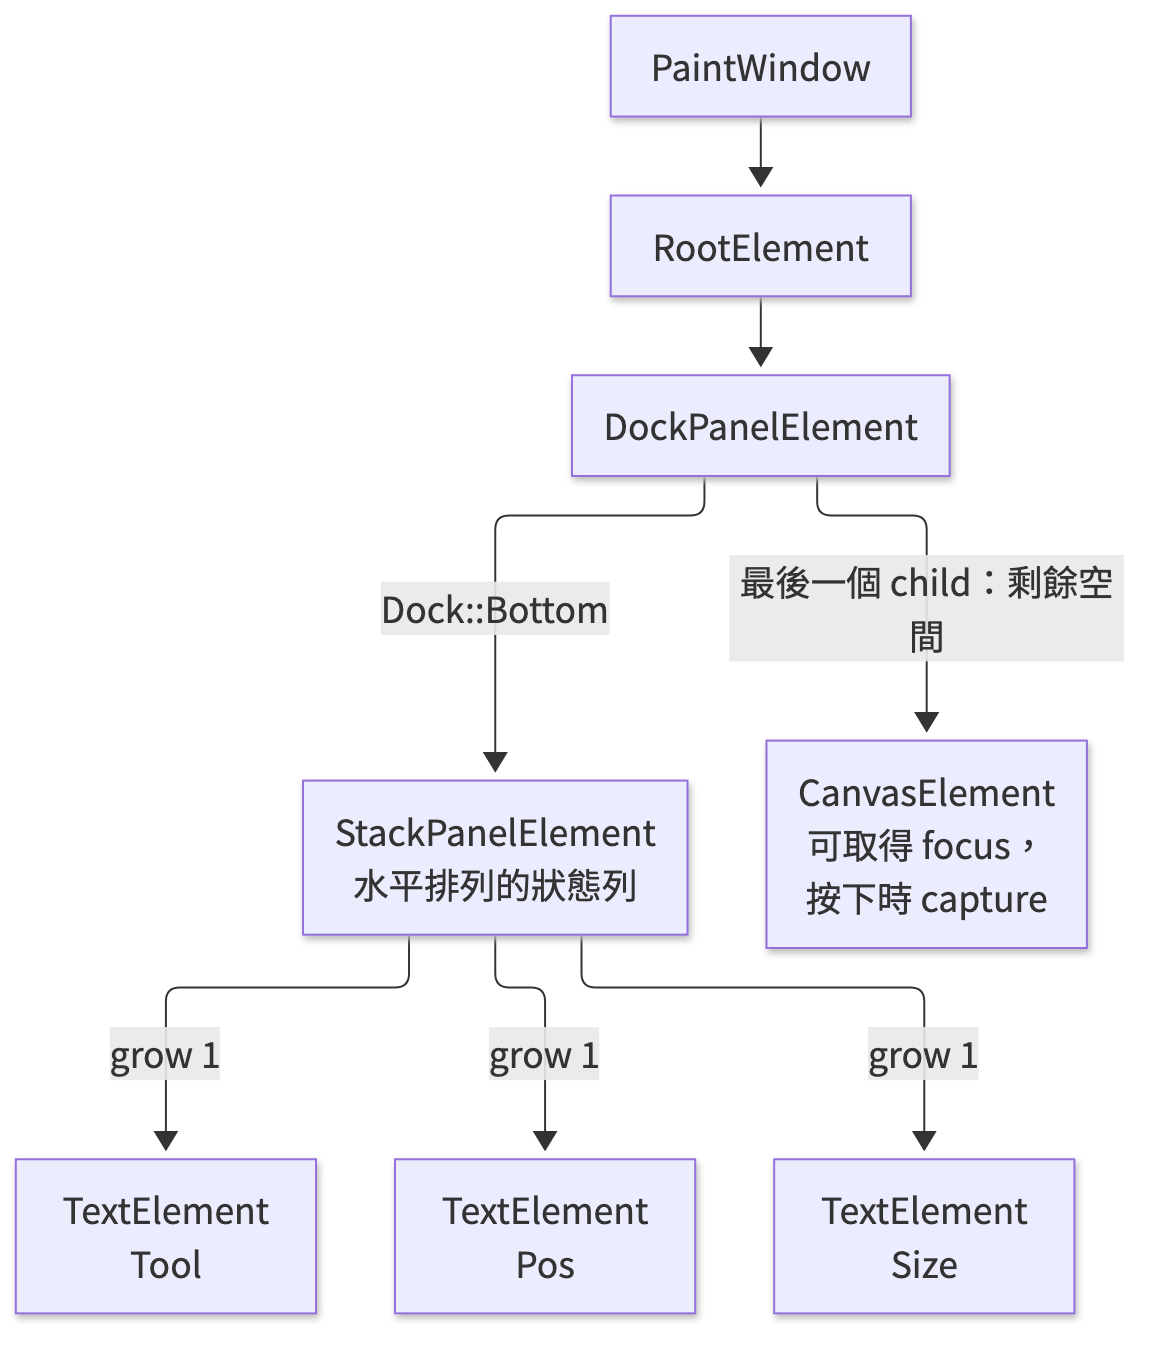
\includegraphics[width=.55\textwidth]{docs/figures/app_a_layout-tree.png}
    \caption{主繪圖視窗的 Element Tree}
    \label{fig:layout-tree}
\end{figure}

\subsection{Layout：Measure 與 Arrange}
\label{app:gui-layout}

版面配置分成兩個遞迴階段。\textbf{Measure} 由父元素傳入可用大小（任一維度可為「不限制」），元素扣除 margin 與 padding 後量測內容，再加回 padding、套用 preferred size，回報包含 margin 的需求大小。\textbf{Arrange} 則由父元素分配實際範圍，元素扣除 margin 後依 alignment（Start、Center、End、Stretch）決定自己的 bounds，再將內容區域交給子元素。bounds 改變時會發出 \lstinline|ElementResizeEvent|，主視窗即藉此同步 Canvas 的大小。

兩種容器的配置規則如下：
\begin{itemize}
    \item \textbf{StackPanel}：沿主軸依序排列，量測時主軸方向不限制，讓子元素回報自然大小。剩餘空間依各子元素的 grow 權重分配；為避免各自取整後遺失像素，程式以累積權重計算每個子元素的邊界，並把餘數交給最後一個有 grow 的子元素。狀態列的三個欄位即以相同權重平分寬度。
    \item \textbf{DockPanel}：子元素依序停靠在剩餘區域的上、下、左、右側，最後一個子元素取得所有剩餘空間。主視窗先將狀態列停靠在底部，再讓 Canvas 填滿其餘區域。
\end{itemize}

屬性改變時，元素只呼叫 \lstinline|invalidateLayout()| 標記版面失效；Window 會在下一次繪製或 Hit Test 前才重新計算整棵樹，避免同一個事件中多次修改而重複配置。

\subsection{事件分派}
\label{app:gui-event}

所有可接收事件的物件都繼承 \lstinline|EventTarget|，以事件型別為 key 保存 listener。\lstinline|dispatchEvent()| 會先記錄 target，再從 target 開始呼叫 listener；若該事件支援 bubbling，便沿著 parent 往上傳遞，Element Tree 的根節點之上則是 Window 本身。傳遞過程中 target 不變，current target 隨所在層級改變，任何一層都可以呼叫 \lstinline|stopPropagation()| 中止傳遞。

事件的 target 依種類決定，如圖~\ref{fig:event-dispatch}：
\begin{itemize}
    \item \textbf{滑鼠事件}：若有元素取得 mouse capture，事件一律送給它；否則以 Hit Test 找到最深層的元素。Canvas、按鈕、色彩區域與 Hue slider 都在按下時 capture、放開時釋放，因此拖曳到元件外仍能收到移動與放開事件。Hover 則永遠依實際位置判斷，不受 capture 影響。
    \item \textbf{鍵盤與文字事件}：送給目前的 focused element，沒有時送給 Window。按下滑鼠時，程式從命中元素沿 parent 往上找最近一個可取得 focus 的元素，並對新舊焦點分別發出 Focus 與 Blur 事件。
\end{itemize}

FreeGLUT 只回報按下與放開，Click 與 DoubleClick 由 Window 自行合成：按下與放開的距離在 4 px 以內才視為 Click，若與上一次 Click 相隔 300 ms 內且位置相近，則改發 DoubleClick，Polygon 工具即以此結束繪製。

\begin{figure}[htbp]
    \centering
    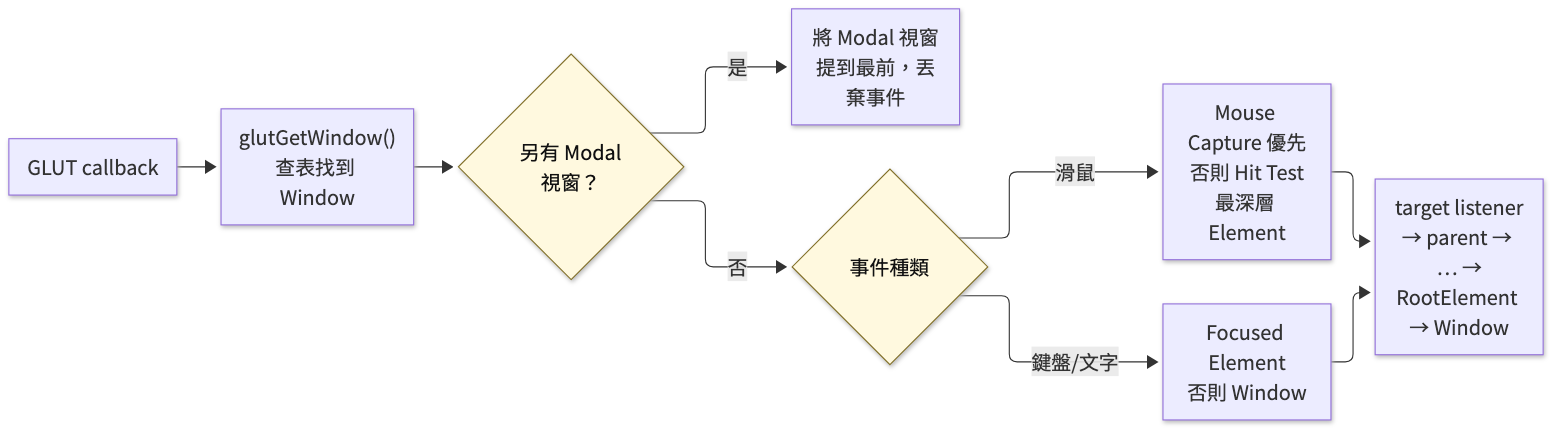
\includegraphics[width=\textwidth]{docs/figures/app_a_event-dispatch.png}
    \caption{GLUT callback 轉為事件後的分派流程}
    \label{fig:event-dispatch}
\end{figure}

\subsection{Window、Modal 與生命週期}
\label{app:gui-window}

GLUT callback 是不帶任何物件的 static function，因此 \lstinline|Window| 以 GLUT 視窗 ID 為 key 維護一張對照表，callback 觸發時以 \lstinline|glutGetWindow()| 查出目前的 Window，再轉交給該物件處理。主繪圖視窗、文字輸入與確認對話框、顏色選擇器，以及 PPM 匯出時使用的視窗，都是 \lstinline|Window| 的子類別。

對話框以 Modal 方式開啟：同一時間只記錄一個 Modal 視窗，開啟時先清除所有視窗的按鍵、點擊與 capture 狀態；之後其他視窗收到鍵盤、滑鼠或選單輸入時，會直接丟棄事件並把 Modal 視窗提到最前面。游標進出視窗時清除滑鼠按鍵狀態，元素被移除時也會一併清除指向該子樹的 focus、hover 與 capture，避免之後把事件送到已經不存在的元素。

視窗關閉通常發生在 callback 執行途中，若立刻釋放物件，callback 返回後可能存取到已刪除的記憶體。因此關閉時只將視窗標記為待關閉，由 \lstinline|Application| 在 GLUT 的 idle callback 中統一釋放。

\subsection{Menu 與 Shortcut}
\label{app:gui-menu}

FreeGLUT 的選單以整數 ID 識別，callback 只會收到被點選項目的 ID。\lstinline|Menu| 將 GLUT 選單包裝成物件，讓每個項目直接對應一個 \lstinline|std::function|，子選單由父選單擁有而形成一棵樹。callback 觸發時先找到所屬的 Menu，確認沒有被 Modal 視窗擋下後，再執行對應項目的動作。

快捷鍵由 \lstinline|ShortcutManager| 管理。每組快捷鍵是一個 key chord，也就是必須同時按住的按鍵與修飾鍵集合；修飾鍵中的 Primary 在 macOS 對應 Command，在其他平台對應 Ctrl，讓同一組綁定能跨平台使用。KeyDown 事件發生時，管理器只考慮包含剛按下按鍵、且所有按鍵都處於按下狀態的 chord，並在多個 chord 同時符合時選擇按鍵數最多的一組，例如按下 Primary+Shift+Z 時執行 Redo，而不是同樣符合的 Primary+Z。按住不放產生的重複事件則會被忽略，避免動作連續觸發。快捷鍵在 Window 層處理，因此鍵盤事件會先送到 focused element，只有元素沒有呼叫 \lstinline|stopPropagation()| 時才會 bubbling 到 Window 並觸發快捷鍵。主視窗中，選單項目與對應的快捷鍵綁定到同一個函式，避免兩邊的行為不同步。
